
Extensive simulation is essential for a new sensor development. 
The  Technology Computer-Aided Design (TCAD) SYNOPSYS was selected  as a tool for simulations, widely used for the development and optimization of semiconductor processing technologies and devices~\cite{Synopsys}. 
In particular, three tools have been exploited: SPROCESS, SDE and SDEVICE. 
%FIXME introduce variable for SPROCESS, SDE, SDEVICE, ...
SPROCESS simulates the fabrication steps in silicon process technologies. 
SDE builds and edits device structures using geometric operations. 
SDEVICE simulates the electrical, thermal, and optical characteristics of silicon and compound semiconductor devices~\cite{SynopsysIncG-2012.06}.

The parameters which should be optimised are the width and depth of implants, distance within/to next layer, position/shift to neighbouring layer,
 the number of layers and optimal doping concentrations for deep implants.
The profile of the electric field yielding an optimal charge sharing is a result of the scan over the mentioned parameters. 

The TCAD geometry of the ELAD sensor Fig. \ref{fig:geo-elfield} (A) contain p-type sensor, three layers of n and p deep implants, p-spray isolation, readout implants, readout electrodes, SiO${}_2$ and backplane. 
With the p-spray isolation technique a shallow unstructured p implant prevents the build-up of an electron layer below the oxide~\cite{Lutz}. 
The p-spray concentration was chosen according to the value of the breakdown voltage~\cite{Pellegrini}. 
The shape of implants is described by using an error function. 
The total sensor thickness is 150 $\muup$m, the pitch size is 55 $\muup$m in agreement with TimePix3~\cite{TimePix}. readout chip, which is foreseen to be used later on. 

\begin{figure}[t]
\begin{minipage}[h]{0.5\linewidth}
\center{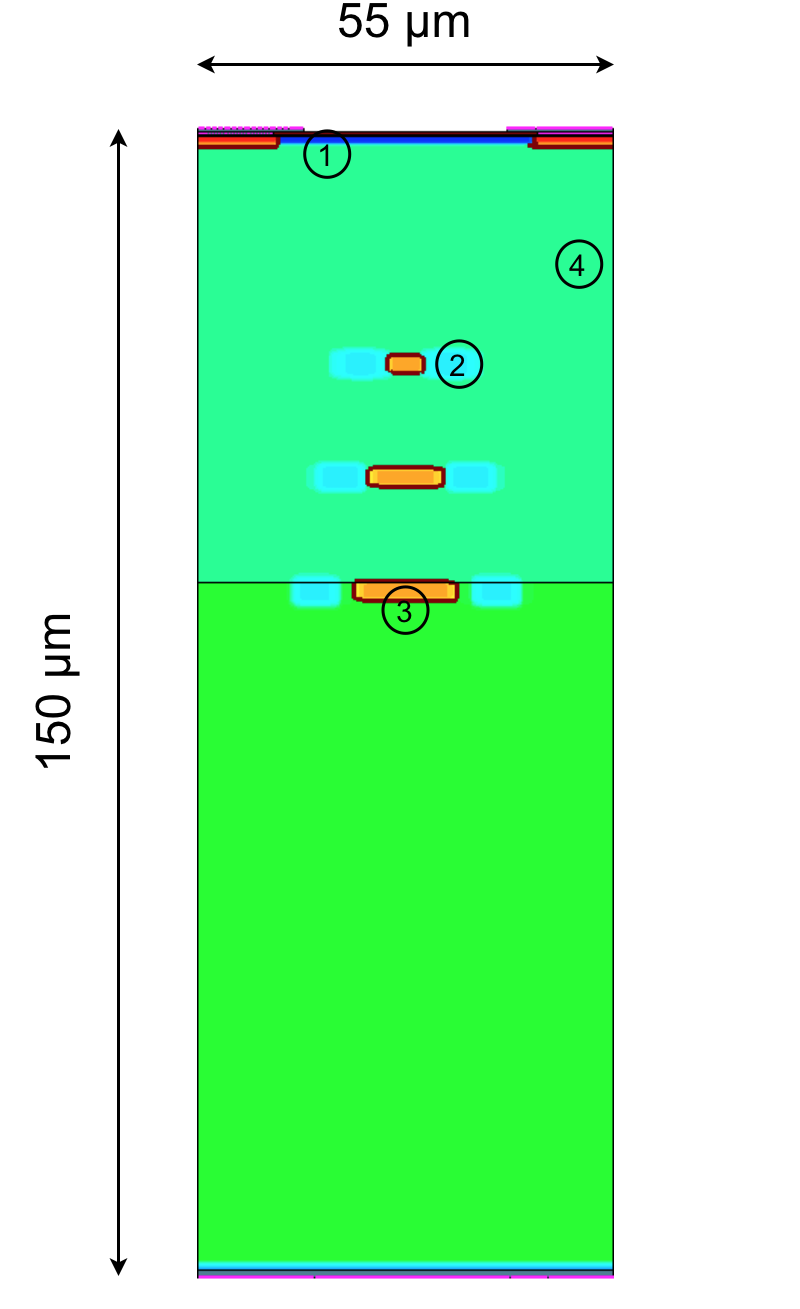
\includegraphics[trim= 0 0 0 0, height=7cm]{pictures/geometry.png} \\ (A)}
\end{minipage}
\hfill 
\begin{minipage}[h]{0.5\linewidth}
\center{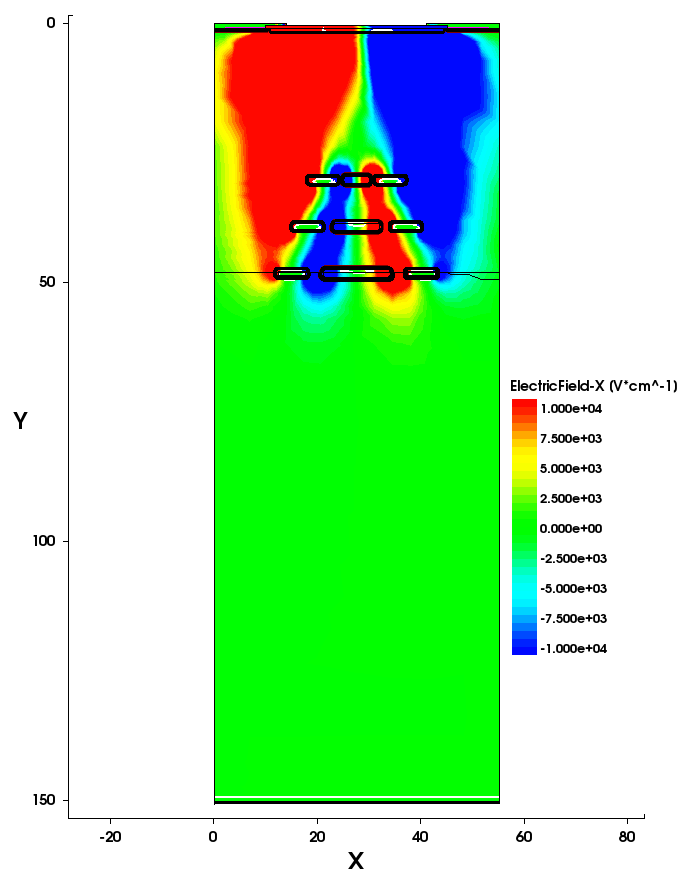
\includegraphics[trim= 0 0 0 0, height=7cm]{pictures/elfield.png} \\(B)}
\end{minipage}
\caption[short description here]
 {(A) TCAD geometry of the ELAD sensor. 1 - p-spray, 2 - deep p-implant, 3 - deep n-implant, 4 - epi-zone. 
 (B) TCAD simulation of the electric field in the ELAD sensor. 
 }
\label{fig:geo-elfield}
\end{figure}

The TCAD simulation of an electric field shows that the p- and n- deep implants lead to cause changes of the potential Fig.~\ref{fig:geo-elfield}~(B). 
The mean electric field is similar to an electric field in a standard design sensor, but the local higher dose implants change the field locally, i.e.\ include an electric field component in $x$ direction. 
The charges drift towards middle between strip/pixel and change their drift path due to diffusion.
Red zones in Fig.~\ref{fig:geo-elfield}~(B) force electrons to change their drift path to the right, blue zones to the left, consequently create the possibility of collecting the charge by two strips. 
In addition the simulation shows that the non-homogeneous electric field in $x$-direction in the ELAD sensor is stable in time. 


\begin{figure}[t]
 \begin{minipage}[h]{0.24\linewidth}
 \center{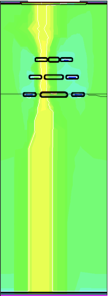
\includegraphics[trim= 0 0 0 0, height=7.5cm]{pictures/driftt1.png} \\ (1)}
 \end{minipage}
 \begin{minipage}[h]{0.24\linewidth}
 \center{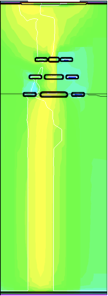
\includegraphics[trim= 0 0 0 0, height=7.5cm]{pictures/driftt2.png} \\(2)}
 \end{minipage}
 \begin{minipage}[h]{0.24\linewidth}
 \center{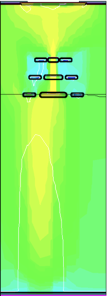
\includegraphics[trim= 0 0 0 0, height=7.5cm]{pictures/driftt3.png} \\(3)}
 \end{minipage}
 \begin{minipage}[h]{0.24\linewidth}
 \center{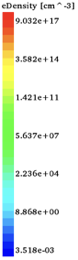
\includegraphics[trim= 0 0 0 0, width=2cm]{pictures/driftscale.png}}
 \end{minipage}
\caption[short description here]
  {TCAD drift simulation in the ELAD sensor. (1) at $t = \SI{e-12}{\sec}$, (2) at $t = \SI{e-10}{\s}$, (3) at $t = \SI{1.2e-9}{\s}$.}
\label{fig:drift}
\end{figure} %FIXME pictures are of bas quality, use high resolution! or at best vector grpahics (eps file)

To understand the behaviour of charge carriers in the ELAD sensor the drift simulation has been carried out. 
It has shown that the charge carriers created near an electrode are collected by it, but the charge created beneath the deep implants area
 changes its drift path and is collected by two strips Fig.~\ref{fig:drift}.  
Thereby, the drift simulation proves that the charge sharing in ELAD sensors is possible on condition of using the non-homogeneous electric field in $x$-direction. 


 